\section{Udvælgelse af gestik-par til at skrue op og ned for musikken}
\label{TestresultaterVolumen}
%
Udvælgelsen af hvilket gestik-par, der skal knyttes til at skrue op og ned for musikken foretages på baggrund af testpersonernes udsagn. I \fullref{app:TestresultaterVolumenDaarlig} analyseres testpersonernes respons i forhold til hvilke gestik-par de mindst kan lide og på baggrund af den analyse ekskluderes gestik-par 6, gestik-par 7 og gestik-par 8 fra yderligere undersøgelser. Dette medfører at udvælgelsen af hvilket gestik-par, der skal knyttes til at skrue op og ned kun foretages på gestik-par 1, gestik-par 2, gestik-par 3, gestik-par 4, gestik-par 5 og gestik-par 9.\blankline
%  
I nedenstående \autoref{tab:GestikParITopTreVolumen} fremgår samtlige testpersoners top tre rangering, hvor der ikke er taget forbehold for hvorvidt testpersonerne har inkluderet et gestik-par, som der på baggrund af \fullref{app:TestresultaterPauseDaarlig} er blevet ekskluderet.
%
\begin{table}[H]
	\centering
	\begin{tabular}{ | p{3cm} | p{3cm} | p{3cm} | p{3cm} |}
		\hline
		& 1. Plads & 2. Plads & 3. Plads \\ \hline
		Testperson 1 & Gestik-par 2 & Gestik-par 6 & Gestik-par 3 \\ \hline
		Testperson 2 & Gestik-par 4 & Gestik-par 5 & Gestik-par 6 \\ \hline
		Testperson 3 & Gestik-par 9 & Gestik-par 4 & Gestik-par 2 \\ \hline
		Testperson 4 & Gestik-par 3 & Gestik-par 1 & Gestik-par 2 \\ \hline
		Testperson 5 & Gestik-par 6 & Gestik-par 1 & Gestik-par 5 \\ \hline
		Testperson 6 & Gestik-par 3 & Gestik-par 4 & Gestik-par 8 \\ \hline 
		Testperson 7 & Gestik-par 2 & Gestik-par 5 & Gestik-par 3 \\ \hline
		Testperson 8 & Gestik-par 1 & Gestik-par 4 & Gestik-par 3 \\ \hline
		Testperson 9 & Gestik-par 9 & Gestik-par 1 & Gestik-par 4 \\ \hline
		Testperson 10 & Gestik-par 3 & Gestik-par 5 & Gestik-par 2 \\ \hline
		Testperson 11 & Gestik-par 3 & Gestik-par 4 & Gestik-par 8 \\ \hline
		Testperson 12 & Gestik-par 4 & Gestik-par 3 & Gestik-par 5 \\ \hline
		Testperson 13 & Gestik-par 3 & Gestik-par 2 & Gestik-par 1 \\ \hline
		Testperson 14 & Gestik-par 2 & Gestik-par 6 & Gestik-par 5 \\ \hline
		Testperson 15 & Gestik-par 3 & Gestik-par 4 & Gestik-par 9 \\ \hline
		Testperson 16 & Gestik-par 1 & Gestik-par 3 & Gestik-par 9 \\ \hline
		Testperson 17 & Gestik-par 2 & Gestik-par 9 & Gestik-par 3 \\ \hline
		Testperson 18 & Gestik-par 4 & Gestik-par 2 & Gestik-par 9 \\ \hline
	\end{tabular}
	\caption{Oversigt over samtlige testpersoners top tre i forbindelse med at skrue op og ned for musikken.}
	\label{tab:GestikParITopTreVolumen}
\end{table}
\noindent
%
Få at få et overblik over hvor ofte de ni forskellige gestik-par individuelt indgår på enten en første, anden eller tredje plads i top tre rangeringen opstilles følgende \autoref{fig:SamletTopTreVolumen}, som bygger på data fra \autoref{tab:GestikParITopTreVolumen}. 
%
\begin{figure}[H]
	\centering
	\includegraphics[resolution=300,width=0.9\textwidth]{Test1/DatabehandlingGrafer/TopTreVolumen}
	\caption{Barplot over hvordan hvert gestik-par indgår i testpersonernes top tre i forhold til at skrue op og ned.}
	\label{fig:SamletTopTreVolumen}
\end{figure}
\noindent
%
Da der er tre gestik-par, som er blevet ekskluderet, kan ovenstående  \autoref{tab:GestikParITopTreVolumen} med fordel opsummeres både i forhold til at fjerne de tre gestik-par men også i forhold til at opsummere hvor mange gange de seks tilbageværende gestik-par indgår i top tre rangeringen. 
%
\begin{table}[H]
	\centering
	\begin{tabular}{ | p{2.4cm} | p{2.4cm} | p{2.4cm} | p{2.4cm} |p{2.4cm}|}
		\hline
		& 1. Plads & 2. Plads & 3. Plads & I alt \\ \hline
		Gestik-par 1 & 2 & 3 & 1 & 6\\ \hline
		Gestik-par 2 & 4 & 2 & 3 & 9\\ \hline
		Gestik-par 3 & 6 & 2 & 4 & 12\\ \hline
		Gestik-par 4 & 3 & 5 & 1 & 9\\ \hline 
		Gestik-par 5 & 0 & 3 & 3 & 6\\ \hline
		Gestik-par 9 & 2 & 1 & 3 & 6\\ \hline
	\end{tabular}
	\caption{Oversigt over dels hvor mange gange hvert gestik-par indgår i samtlige testpersoners top tre i forbindelse med at skrue op og ned for musikken og dels over hvor mange gange et gestik-par sammenlagt indgår i en top tre.}
	\label{tab:GestikParITopTreVolumenOversigt}
\end{table}
\noindent
%
De to testpersoner, som begge har tildelt gestik-par 1 en første plads forbinder bevægelsen med noget de er vant til; at dreje på en knap for at skrue op. Gestik-par 1 illustreres på \autoref{fig:GestikPar1Volumen}. Derudover påpeger testperson, 8 at i forhold til bevægelsen i gestik-par 2 så er gestik-par 1 tydeligere og at gestik-par 1 er naturlig. Gestik-par 2 illustreres på \autoref{fig:GestikPar2Volumen}. I tillæg påpeger testperson 16, at bevægelsen i gestik-par 1 så mere behagelig ud sammenlignet med gestik-par 2, som testpersonen fandt ukomfortabel. En af årsagerne til at testperson 16 vurderer at gestik-par 2 er ukomfortabel skyldes formentlig, at i videooptagelsen bliver gestik-par 2 ikke gengivet lige så afslappet, som det var hensigten. I videooptagelsen fremgår det at nærmest hele armen skal i bevægelse; fra skulderen og ud til fingrene, hvilket ikke er hensigten med gestikken. Hensigten med gestik-par 2 er, at bevægelsen bør dannes ud fra en kombination mellem underarmen, håndleddet og fingrene, så det tilnærmelsesvist er den samme bevægelse, som går igen ved gestik-par 1. Sammenholdes testperson 16’s udsagn med testpersonens bevægelser, når testpersonen opfordres til at komme med et forbedringsforslag, så begynder testpersonen rent faktisk med at gengive bevægelsen i gestik-par 2 og det er først når testlederen konfronterer testperson 16, at testpersonen gengiver gestik-par 1. Når testperson 16 afslutningsvist bliver bedt om, at gengive sine foretrukne gestikker, så er det heller ikke gestik-par 1 testpersonen gengiver men starten på gestik-par 2, illustreret på \autoref{fig:GestikPar2Volumen}, og når der så skrues op eller ned gøres det med en flad og udstrakt hånd i en cirkulærbevægelse. Sammenholdes det testpersonen giver udtryk for, med hvad testpersonen rent faktisk gør, så stemmer det ikke overens i forhold til gestik-par 1, som illustreres på \autoref{fig:GestikPar1Volumen}. Det tyder derfor på, at testpersonen formentligt foretrækker noget, der tilnærmelsesvist minder om gestik-par 2, men særligt foretrækker en cirkulærbevægelse.
%
\begin{figure}[H]
	\centering
	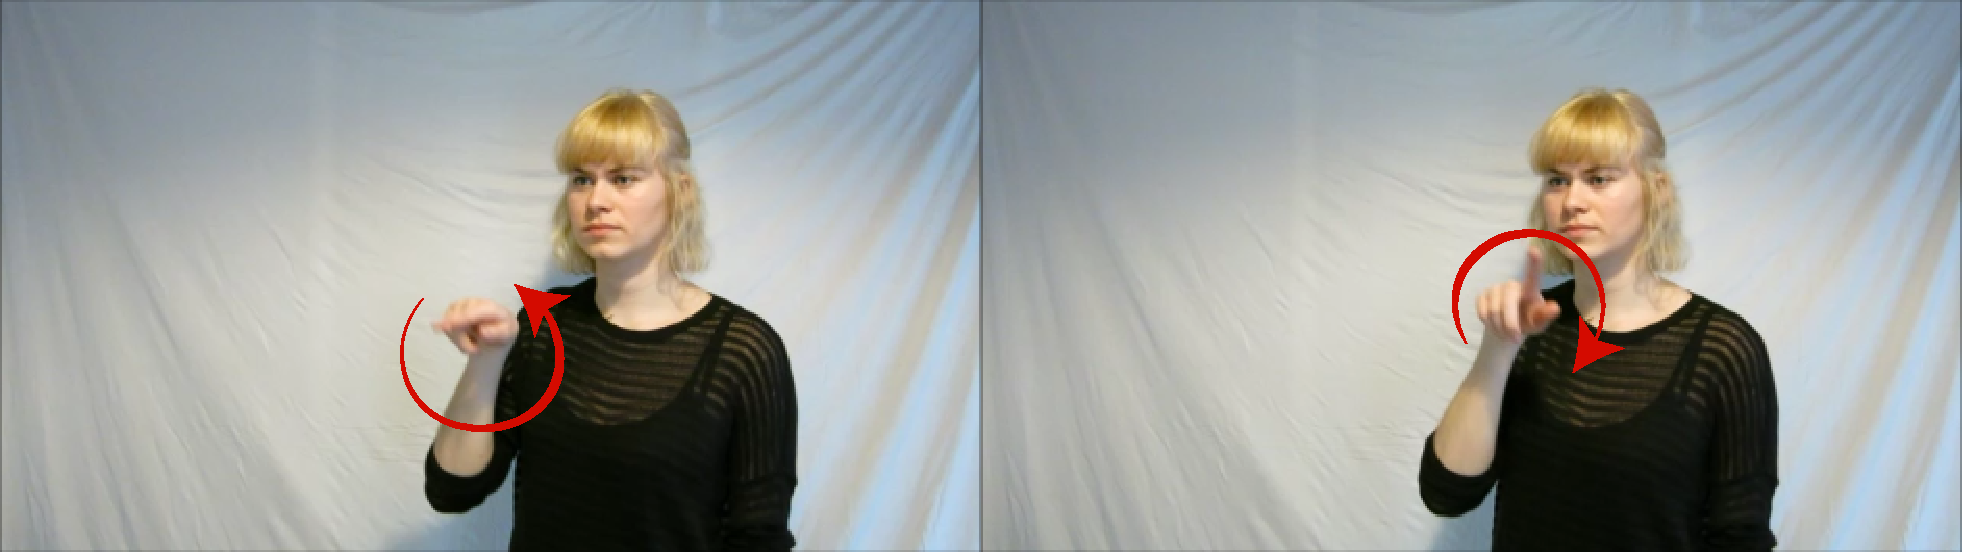
\includegraphics[resolution=300,width=0.9\textwidth]{Test1/Gestik-par/Gestik1_Volumen}
	\caption{Illustration af gestik-par 1; cirkulærbevægelse med pegefingeren i urets retning for at skrue op og mod uret for at skrue ned.}
	\label{fig:GestikPar1Volumen}
\end{figure}
\noindent
%
Baseret på testperson 4’s udsagn, så tyder det ikke på, at der er en særlig årsag til at gestik-par 1 er rangeret højere end gestik-par 2. Testpersonen giver udtryk for, at det er en naturlig bevægelse og at det er det testpersonen tænker, når der skal skrues op eller ned for noget. Testperson 5 giver udtryk for, at gestik-par 1 er intuitiv, nem at forstå, det er universelt så alle kan gengive bevægelsen, bevægelsen kan laves overalt og i forskellige størrelser. Derudover pointerer testpersonen, at gestik-par 1 er hurtigere at gengive end gestik-par 2. Dog giver testperson 5 først udtryk for, at kunne lide, hvad testpersonen definerer som volumen-knappen, svarende til gestik-par 2, som illustreres på \autoref{fig:GestikPar2Volumen}. Årsagen til at gestik-par 2 ikke indgår i testpersonens top tre, er fordi testpersonen finder den langsom at gengive. Testperson 9 tildeler først gestik-par 1 en første plads, men efter at have prøvet det tildeler testpersonen gestik-par 9 første pladsen. Gestik-par 9 illustreres på \autoref{fig:GestikPar9Volumen}. Testpersonen giver udtryk for, at foretrække gestikker, som kun kræver én hånd og som ikke distraherer testpersonens barn. Derudover kommenterer testpersonen, at gestik- par 1 virkede forholdvis overskuelig og nem. Ifølge testperson 9 fravælges gestik-par 2 fordi bevægelsen var stor og klodset, hvilket indikerer at hensigten med gestik-parret igen er fejlfortolket.

Med udgangspunkt i testperson 13’s udsagn er det ikke entydigt hvorfor testpersonen har tildelt gestik-par 1 en trejde plads, men testpersonen giver udtryk for, at de cirkulærebevægelser er sjove og at det minder om en knap. Derudover foretrækker testpersonen ligeledes, at gestikkerne kun kræver én hånd.
%
\begin{figure}[H]
	\centering
	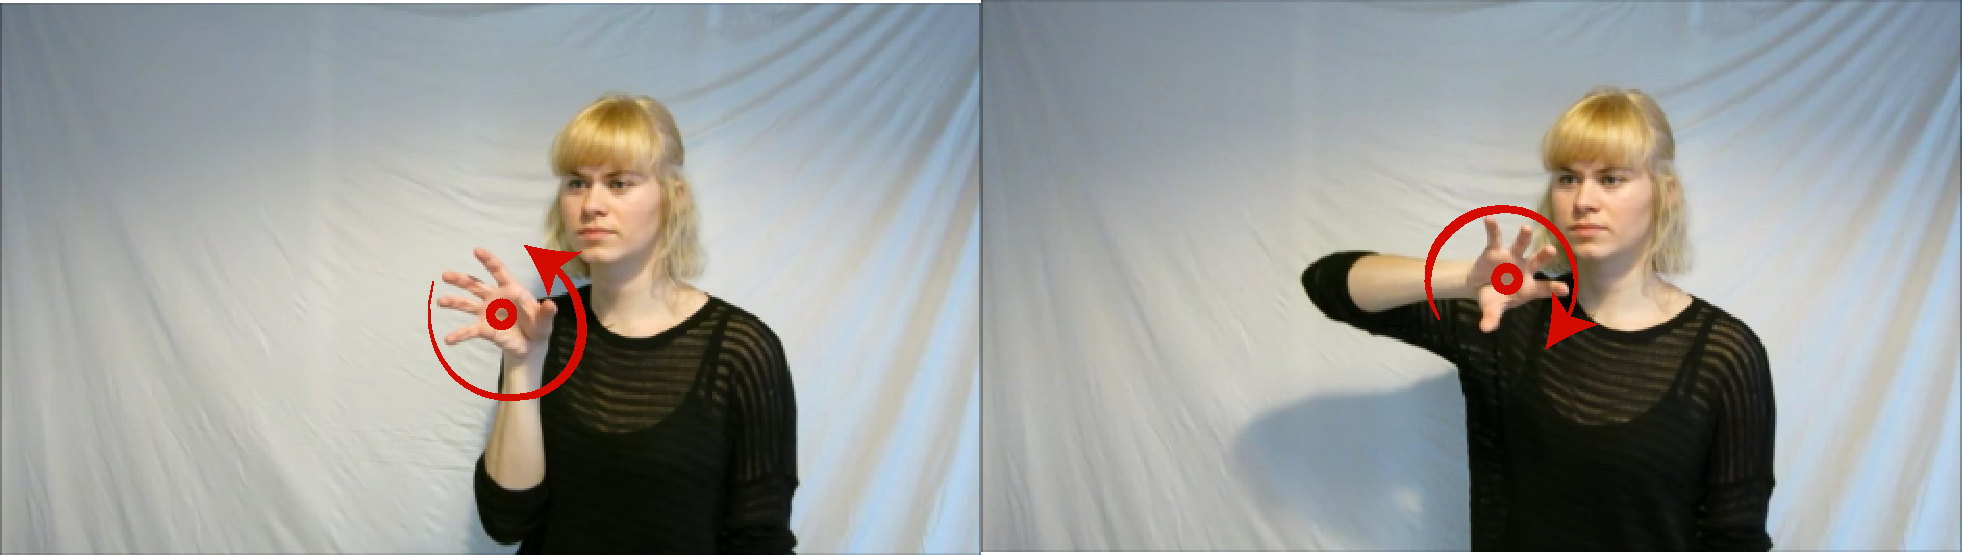
\includegraphics[resolution=300,width=0.9\textwidth]{Test1/Gestik-par/Gestik2_Volumen}
	\caption{Illustration af gestik-par 2; cirkulærbevægelse med halv bøjede fingrene, ligesom hvis det var en dreje-knap, der blev brugt. Der skal drejes med uret for at skrue op og mod uret for at skrue ned.}
	\label{fig:GestikPar2Volumen}
\end{figure}
\noindent
%
Seks ud af de ni testpersoner, som har inkluderet gestik-par 2 i sin top tre, forbinder gestikken med en drejeknap, som de i forvejen er vant til at interagere med for at skrue op eller ned på et anlæg, jævnfør \autoref{fig:GestikPar2Volumen}. Tre ud af de fire, som har tildelt gestik-par 2 en første plads, kommenterer, at de finder bevægelsen naturlig. Ifølge testperson 1, så tænkte testpersonen på gestik-par 2 allerede før testpersonen blev præsenteret for gestik-parret. Både testperson 17, testperson 18 og testperson 3 giver udtryk for, at bevægelsen giver mening for at skrue op eller ned for musikken. Igen vælger testperson 14 gestikker ud fra hvad der ikke naturligt forekommer, når testpersonen normalvist gestikulerer, hvorfor testpersonen har tildelt gestik-par 2 en første plads. Lignende argumenter fremsættes af testperson 18, som påpeger at bevægelsen i gestik-par 2 er så specifik, at det ikke er en bevægelse, der fejlagtigt opstår, jævnfør \autoref{fig:GestikPar2Volumen}. Derudover kommenterer testperson 18, at det er behageligt at dreje lyden op. Ligesom det er nævnt ved gestik-par 1, så giver testperson 13 udtryk for dels at cirkulærbevægelser er sjove og dels foretrækker en-hånds gestikker. Ifølge testperson 10, så er gestik-par 2 både intuitiv og nem at huske.

Udover at bevægelsesmængden i gestik-par 2 ikke behøver, at være så udtryksfuld, som det blev illustreret i videooptagelser, så er det kun to testpersoner, som har forbedringsforslag. Testperson 14 foreslår, at den ikke-dominante hånd, altså hånden, som ikke skal foretage cirkelbevægelsen, inkluderes, så det kræver begge hænder at skrue op og ned. I og med at størstedelen af testpersonerne foretrækker gestikker, som kun kræver én hånd, afvises foreslaget, men det tages til eftertrakning, at der måske skal være et nyt element i gestik-par 2. Et forslag til det fremsættes af testperson 1, som foreslår at hånden først er lukket sammen i en knytnæve og når hånden åbnes, så kan bevægelserne i gestik-par 2 udføres. Det nye element i gestik-par 2 behøver ikke nødvendigvis at være en lukket knytnævne, men kan være en indikation af, at brugeren tager fat i en drejeknap, da flere testpersoner forbinder gestik-par 2 med dette.  

En af fordelene ved at vælge gestik-par 2 fremfor gestik-par 1 er, at gestik-par 2 oftere indgår i testpersonernes samlede top tre, jævnfør \autoref{tab:GestikParITopTreVolumenOversigt}. Det anses ydermere for at være en fordel, at flere testpersoner forbinder bevægelsen i gestik-par 2 med noget de i forvejen er vant til, fordi de så ikke nødvendigvis behøver at lære noget nyt. Derudover antages det, at størstedelen af de personer, som har \textit{high-end} lydudstyr formentlig også har en forstærker, hvorpå lydstyrken normalvist ændres ved at dreje på en drejeknap, hvilket formentlig vil gøre det lettere for brugeren, at koble gestik-par 2 til den funktion. Ydermere påpeger både testperson 14 og testperson 18, at bevægelsen i gestik-par 2 ikke er en bevægelse, der normalvist indgår i ens naturlige gestikulation. Med forbehold for, at gestik-par 2 ikke nødvendigvis skal gengives på præcis samme måde, som det fremgår i videooptagelsen og at der muligvis først skal være en indikation af, at nu skal der skrues op eller ned, så vurderes det, at gestik-par 2 egner sig bedre end gestik-par 1 til at skrue op og ned.
%
\begin{figure}[H]
	\centering
	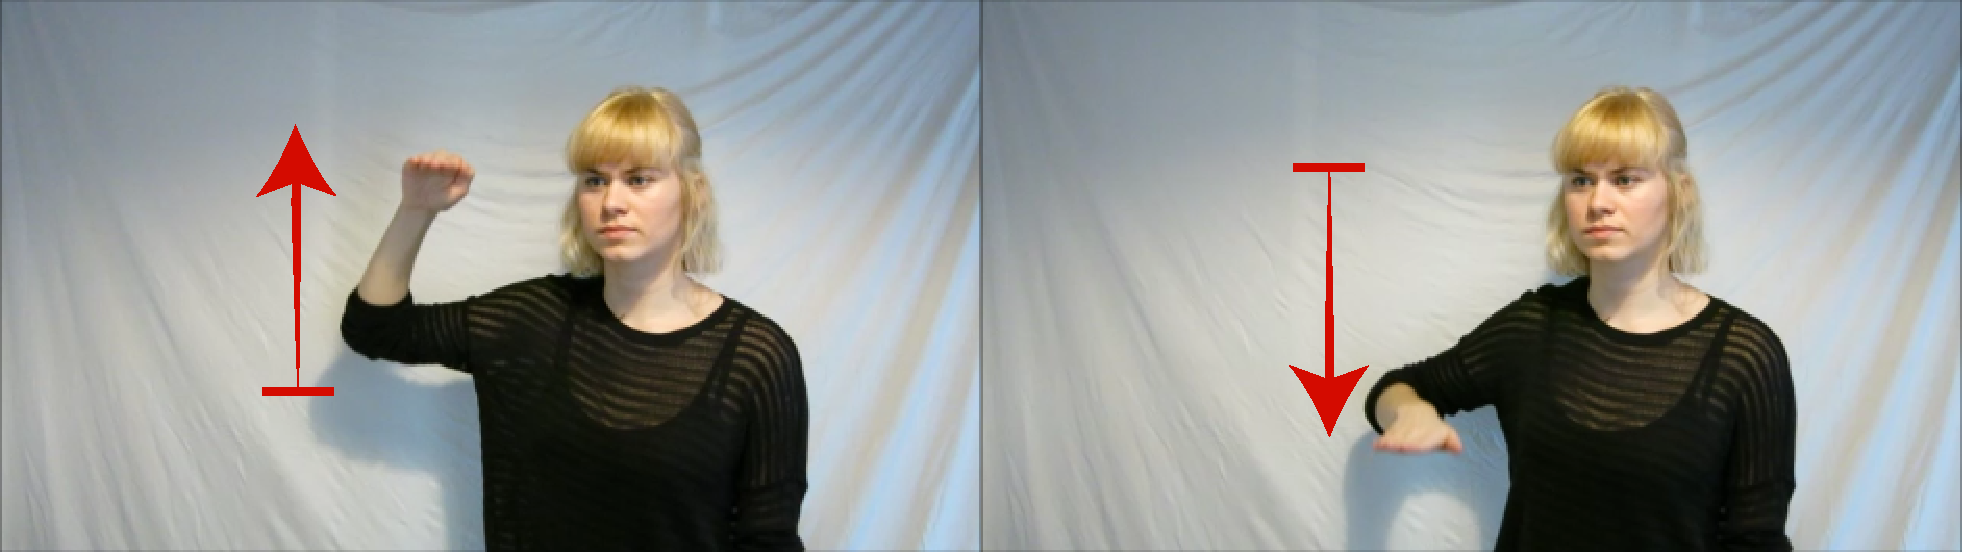
\includegraphics[resolution=300,width=0.9\textwidth]{Test1/Gestik-par/Gestik3_Volumen}
	\caption{Illustration af gestik-par 3; horisontal hånd løftes vertikalt med håndfladen nedad for at skrue op og for at skrue ned sænkes hånden vertikalt med håndfladen nedad.}
	\label{fig:GestikPar3Volumen}
\end{figure}
\noindent
%
På \autoref{fig:SamletTopTreVolumen} fremgår det, at gestik-par 3 er det gestik-par, som sammenlagt indgår flest gange i testpersonernes top tre; 12 gange i alt. På \autoref{fig:GestikPar3Volumen} illustreres gestik-par 3. Det tyder på, at ligesom ved de to foregående gestik-par, så foretrækker de testpersoner, som har tildelt gestik-par 3 en første plads, ligeledes at bevægelsen kan gøres med én hånd. Testperson 4 har tildelt gestik-par 3 en første plads ud fra, hvad der passede godt til det testpersonen valgte til pause og start, hvilket var gestik-par 1, jævnfør \autoref{fig:GestikPar1Volumen}. I og med at det gestik-par blev sorteret fra til pause og start, så er det ikke sikkert, at testpersonen stadig vil tildele gestik-par 3, til at skrue op og ned, en første plads. Testperson 10 giver, foruden at gestik-par 3 er intuitiv og nem at huske, udtryk for, at bevægelsen passer godt til det den skal gøre. Lignende tendens går igen ved testperson 11; som foruden at vurdere gestik-par 3 som værende både logisk og intuitiv, giver udtryk for, at hvis der skal skrues op, så bør det være med en opadgåendebevægelse. Ifølge testperson 6 er både gestik-par 3 og gestik-par 4 naturlige og nemmere at udføre, i forhold til hvis der skal være en bestemt reference, som der blandt andet er i gestik-par 5, jævnfør \autoref{fig:GestikPar5Volumen}. Testperson 13 har svært ved uddybe hvorfor gestikkerne er rangeret i den rækkefølge, som fremgår af \autoref{tab:GestikParITopTreVolumen}, men testpersonen giver udtryk for godt, at kunne lide de gestik-par, hvor hånden enten skal hæves eller sænkes for at skrue op og ned. Både testperson 6 og testperson 13 giver udtryk for, at det er nemt at udføre bevægelserne i gestik-par 3. I tillæg kommenterer testperson 15, at gestik-par 3 er simpel. Disse synspunkter går igen ved testperson 12, som har tildelt gestik-par 3 en anden plads, jævnfør \autoref{tab:GestikParITopTreVolumen}. Ydermere giver testperson 16 og testperson 1 udtryk for, at gestik-par 3 giver mening. Dog tyder det på, at testperson 16 ikke kan huske sin top tre, da testpersonen bliver nødt til at spørge testlederen. Testperson 1, som har tildelt gestik-par 3 en tredje plads, forbinder gestikken med hvordan lyd visualiseres på en computer, hvor testperson 8 giver udtryk for, at det er den gestik, der bruges til at dirigere et kor. Ifølge testperson 7, så har testpersonen tildelt gestik-par 3 en tredje plads, fordi gestik-parret er en kombination af gestik-par 5, jævnfør \autoref{fig:GestikPar5Volumen}, og gestik-par 9, jævnfør \autoref{fig:GestikPar9Volumen}, i forhold til hvor meget kontrol testpersonen har. Testperson 17 kommenterer ikke på hvorfor gestik-par 3 indgår i top tre rangeringen.

Ud af de seks testpersoner, som har tildelt gestik-par 3 en første plads, er der ingen af dem, der begår fejl når de gengiver bevægelsen. Udover at bevægelserne gerne må udføres mere afslappet end hvad der er gengivet på \autoref{fig:GestikPar3Volumen}, så har ingen testpersoner forbedringsforslag. Baseret på foregående analyse vedrørende gestik-par 3, der illustreres på \autoref{fig:GestikPar3Volumen}, så er der på nuværende tidspunkt ikke belæg for, at ekskludere dette gestik-par.
%
\begin{figure}[H]
	\centering
	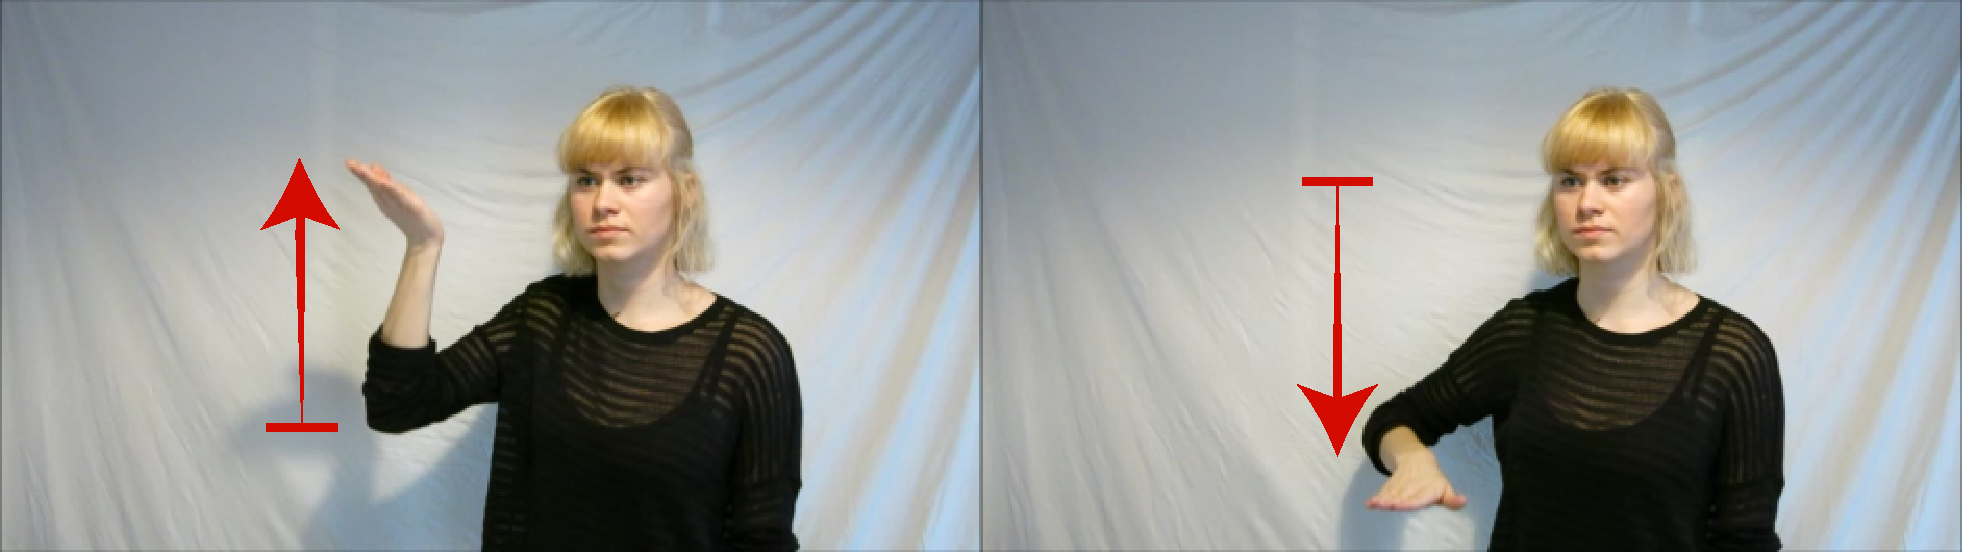
\includegraphics[resolution=300,width=0.9\textwidth]{Test1/Gestik-par/Gestik4_Volumen}
	\caption{Illustration af gestik-par 4; horisontal hånd løftes vertikalt med håndfladen opad for at skrue op og for at skrue ned sænkes hånden vertikalt med håndfladen nedad.}
	\label{fig:GestikPar4Volumen}
\end{figure}
\noindent
%
To ud af tre testperson, som har tildelt gestik-par 4 en første plads, giver udtryk for at bevægelsen giver mening. Gestik-par 4 illustreres på \autoref{fig:GestikPar4Volumen}. Testperson 2 begrunder yderligere sit valg med, at der er en tydelig indikation af hvad der er op og ned.  I tillæg kommenterer testperson 2, at gestik-par 4 er simpel, hvilket testperson 18 ligeledes giver udtryk for. Testperson 18 giver ydermere udtryk for, at årsagen til at gestik-par 4 er på en første plads skyldes, at armen ikke skal være på en bestemt måde, men bare løftes op eller ned. Som tidligere nævnt giver testperson 12 udtryk for, at foretrække gestikker, der kun kræver én hånd, hvilket ligeledes gør sig gældende ved gestik-par 4, jævnfør \autoref{fig:GestikPar4Volumen}. 

Fire ud af fem testperson, som har tildelt gestik-par 4 en anden plads, kommenterer, at det minder om gestik-par 3, jævnfør \autoref{fig:GestikPar3Volumen}. Dog kommenterer testperson 11 og testperson 15 henholdsvis, at der ikke bør skelnes mellem gestik-par 3 og gestik-par 4 og at gestik-par 4 er mere kompliceret end gestik-par 3. Derudover giver testperson 3 udtryk for, at det giver meningen at løfte et eller andet op, i det her tilfælde lydstyrken, og derefter skubbe det ned igen, hvorfor en lodret bevægelse giver mest mening. Ydermere beskriver testperson 11 og testperson 15 gestik-par 4 med ord som; intuitiv, logisk og simpel. Den eneste testperson, som har tildelt gestik-par 4 en trejde plads, er testperson 9. Testpersonen sammenligner gestik-par 4 med gestik-par 9, som illustreres på \autoref{fig:GestikPar9Volumen}. Derudover lægger testperson 9 vægt på hvad der er mindst krævende og mindst distraherende. 

Med udgangspunkt i på testpersonernes udsagn og at gestik-par 4 indgår ni gange i testpersonernes samlede top tre rangering, jævnfør \autoref{tab:GestikParITopTreVolumenOversigt}, så forefinder der på nuværende tidspunkt ikke belæg for, at ekskludere dette gestik-par.  
%
\begin{figure}[H]
	\centering
	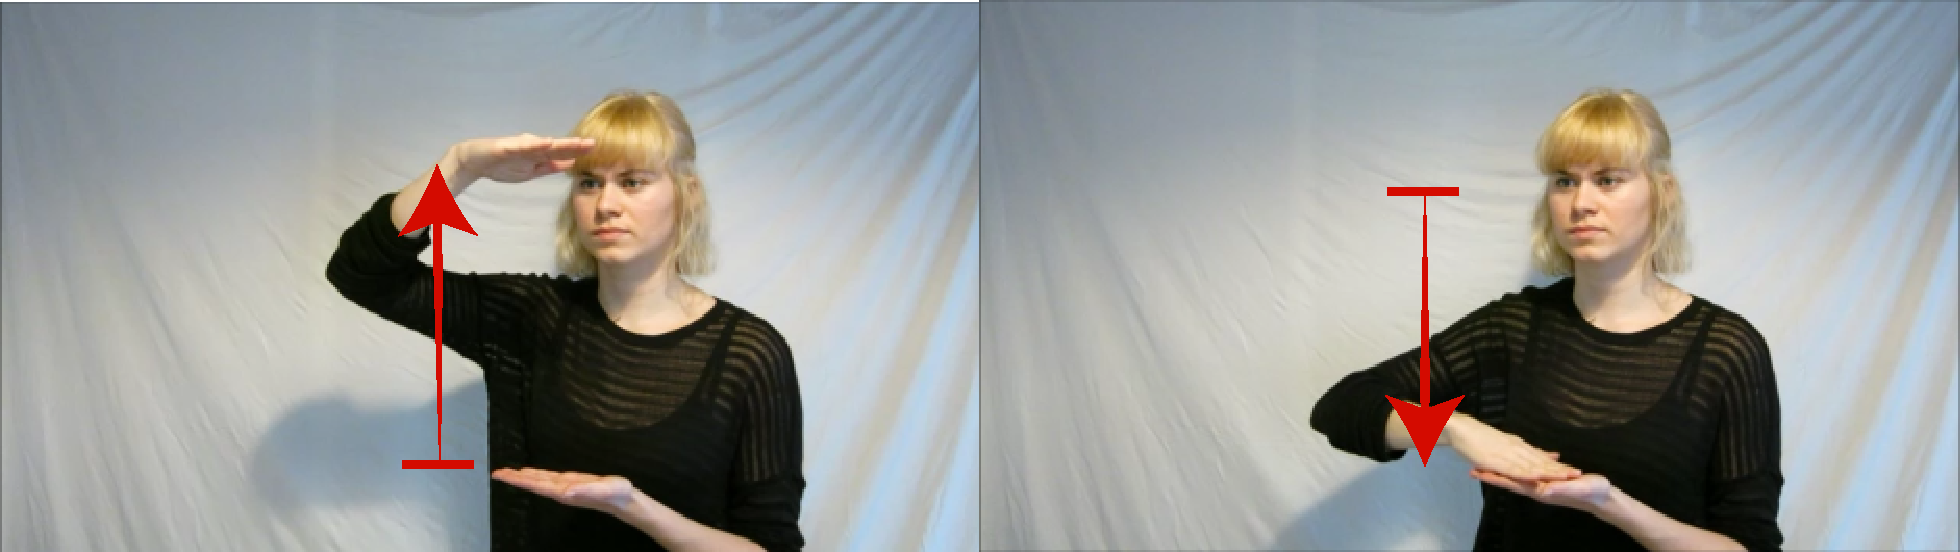
\includegraphics[resolution=300,width=0.9\textwidth]{Test1/Gestik-par/Gestik5_Volumen}
	\caption{Illustration af gestik-par 5; horisontal ikke-dominant hånd med håndfladen opad holdes stationær, mens den dominante hånd ligeledes holde horisontal med håndfladen nedad men løftes vertikalt væk fra den ikke-dominante hånd for at skrue op og sænkes mod den ikke-dominante hånd for at skrue ned.}
	\label{fig:GestikPar5Volumen}
\end{figure}
\noindent
%
Fra \autoref{fig:SamletTopTreVolumen} fremgår det, at gestik-par 5 ikke tildeles en første plads, en eneste gang. Gestik-par 5 illustreres på \autoref{fig:GestikPar5Volumen}. Ifølge testperson 5, så er det nemmere, at kontrollere hvor meget lydstyrken skal ændres, hvis gestikken indeholder to hænder. Lignende kommer til udtryk ved testperson 7. Dog påpeger testperson 5, at testpersonen føler sig mere udsat ved gestik-par 5 sammenlignet med gestik-par 6, som er den samme bevægelse bare horisontalt. Foruden det testperson 10 og testperson 12 har givet udtryk for ved gestik-par 3, så præciserer de ikke nærmere hvorfor de har inkluderet gestik-par 5. Lignende går igen ved testperson 2, som heller ikke præciserer sit valg nærmere. 

Som nævnt tidligere, så foretrækker størstedelen af testpersonerne én-hånds gestikker, hvilket i sig selv er et godt argument for, at ekskludere gestik-par 5. Derudover indgår gestik-par 5 sammenlagt kun seks gange i testpersonernes samlet top tre og aldrig på en første plads, jævnfør \autoref{tab:GestikParITopTreVolumenOversigt}. Ydermere påpeger testperson 6 et potentielt problem ved gestik-par 5; hvis gestikken startes på den lydstyrke, som musikken allerede spiller ved, svarende til at hænderne er samlet, når der så skrues op øges afstanden mellem hænderne og når der skrues ned igen, så ender lydstyrken på hvad den oprindeligt var. Så hvis testpersonen gerne vil skrue endnu mere ned, så opstår der tvivl i hvordan det gøres; skal den dominante hånd så være referencen mens den ikke-dominante hånd angiver hvor meget der skrues ned. Tages alt dette i betragtning vurderes det, at der er belæg for at ekskludere gestik-par 5.      
%
\begin{figure}[H]
	\centering
	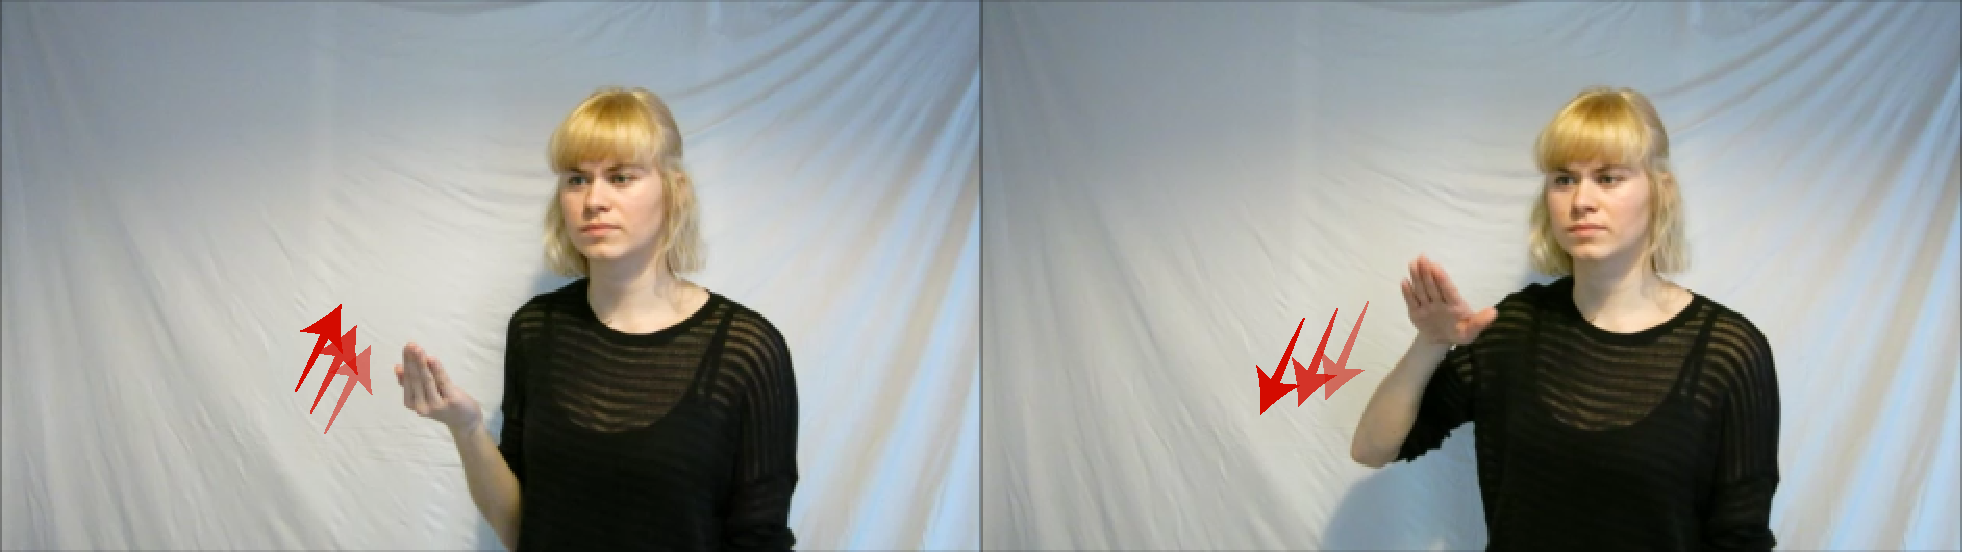
\includegraphics[resolution=300,width=0.9\textwidth]{Test1/Gestik-par/Gestik9_Volumen}
	\caption{Illustration af gestik-par 9; \enquote{Kom så}-bevægelse med fingrene for at skrue op og \enquote{Ro på}-bevægelse med fingrene for at skrue ned.}
		\label{fig:GestikPar9Volumen}
\end{figure}
\noindent
%
Den gennemgående tendens for, at testpersonerne vælger gestik-par 9 er, at den er smart. Gestik-par 9 illustreres på \autoref{fig:GestikPar9Volumen}. De to testpersoner, som har tildelt gestik-par 9 en første plads, begrunder det yderligere med, at det ifølge testperson 3 er meget sejt og ifølge testperson 9 er det naturligt. At gestik-par 9 er naturlig giver testperson 17 ligeledes udtryk for. Derudover beskrives gestik-par 9, som værende; logisk, hurtig, simpel og nem. Endvidere har hverken testperson 3 eller testperson 9 givet udtryk for forbedringer til gestik-par 9, men i begge tilfælde har testpersonerne oprindeligt valgt et andet gestik-par ind til de gengiver bevægelserne og begge konkluderer, at gestik-par 9 skal tildeles første pladsen.

Med udgangspunkt i testpersonernes argumenation for hvorfor de har valgt gestik-par 6 og taget i betragtning af, at gestik-par 9 sammenlagt indgår seks gange i testpersonernes samlede top tre, jævnfør \autoref{tab:GestikParITopTreVolumenOversigt} samt at gestik-parret er fravalgt to gange, jævnfør \autoref{app:TestresultaterVolumenDaarlig}, så vurderes det, at der er belæg for at ekskludere gestik-par 9. Ydermere påpeger testperson 7, at ved gestik-par 9 er der ingen kontrol over lydstyrken, så det kan være hvilken som helst lydstyrke testpersonen ender på ved gestik-par 9. \blankline
%
Baseret på foregående analyse af hvilket semaforisk gestik-par, der skal knyttes til at skrue op og ned for musikken, er det ikke muligt, at udpege et enkelt gestik-par. Valget står mellem gestik-par 2, gestik-par 3 og gestik-par 4, illustreret på henholdvis \autoref{fig:GestikPar2Volumen}, \autoref{fig:GestikPar3Volumen} og \autoref{fig:GestikPar4Volumen}. Fordelen ved at vælge gestik-par 2 er, at det ikke er en bevægelse, som normalvist indgår i ens kropsprog, hvorfor det forventes at sandsynligheden for, at bevægelsen laves ved en fejl er mindre end ved både gestik-par 3 og gestik-par 4. En anden fordel ved at vælge gestik-par 2 er, at størstedelen af testpersonerne forbinder gestikken med noget de er vant til i forvejen; netop at skrue op og ned på et anlæg via en drejeknap. I denne sammenhæng vælges det derfor, at knytte gestik-par 2 til at skrue op og ned.   




     


